\documentclass[11pt,a4paper,oneside]{article}
\usepackage{amsmath,amssymb}
\usepackage[a4paper,left=23mm,right=23mm,top=21mm,bottom=21mm,
  headheight=0pt,headsep=0pt,footskip=10mm]{geometry}
\usepackage{graphicx,array,booktabs,tabularx,float,caption,microtype}
\usepackage[hidelinks,bookmarksnumbered]{hyperref}
\hypersetup{pdftitle={Investment and chronological operation of electricity storage and electrolysis},
  pdfauthor={Group 15}}
\setlength{\parindent}{1em}
\setlength{\parskip}{2pt plus .5pt}
\setlength{\intextsep}{6pt plus 1pt minus 1pt}
\setlength{\textfloatsep}{7pt plus 1pt minus 1pt}
\setlength{\tabcolsep}{4pt}
\setlength{\emergencystretch}{1em}
\renewcommand{\arraystretch}{1.10}
\captionsetup{font=small,labelfont=bf,labelsep=period,skip=4pt}
\newcolumntype{Y}{>{\raggedright\arraybackslash}X}
\newcolumntype{P}[1]{>{\raggedright\arraybackslash}p{#1}}
\newcounter{chapter}
\renewcommand{\thechapter}{\Roman{chapter}}
\renewcommand{\thesection}{\arabic{section}}
\renewcommand{\thesubsection}{\arabic{section}.\arabic{subsection}}
\makeatletter
\@addtoreset{section}{chapter}
\@addtoreset{equation}{chapter}
\@addtoreset{table}{chapter}
\@addtoreset{figure}{chapter}
\newcommand{\chapter}{\@ifstar\academicchapterstar\academicchapter}
\newcommand{\academicchapter}[1]{\clearpage\refstepcounter{chapter}
  \addcontentsline{toc}{chapter}{\protect\numberline{\thechapter}#1}
  \academicchapterhead{#1}}
\newcommand{\academicchapterstar}[1]{\clearpage\academicchapterstarhead{#1}}
\newcommand{\academicchapterhead}[1]{\vspace*{0pt}{\parindent\z@\centering
  \normalfont\Large\bfseries\thechapter.\enspace #1\par}\vspace{9pt}}
\newcommand{\academicchapterstarhead}[1]{\vspace*{0pt}{\parindent\z@\centering
  \normalfont\Large\bfseries #1\par}\vspace{9pt}}
\newcommand{\l@chapter}[2]{\vskip5pt{\bfseries
  \@dottedtocline{0}{0em}{2em}{#1}{#2}}}
\renewcommand{\l@section}{\@dottedtocline{1}{1.8em}{1.8em}}
\renewcommand{\l@subsection}{\@dottedtocline{2}{3.6em}{2.6em}}
\renewcommand{\tableofcontents}{\chapter*{\contentsname}\@starttoc{toc}}
\renewcommand\section{\@startsection{section}{1}{\z@}
  {-8pt plus -2pt}{4pt}{\normalfont\large\bfseries}}
\renewcommand\subsection{\@startsection{subsection}{2}{\z@}
  {-6pt plus -1pt}{3pt}{\normalfont\normalsize\bfseries}}
\def\p@section{\thechapter.}
\def\p@subsection{\thechapter.}
\makeatother
\renewcommand{\theequation}{\thechapter.\arabic{equation}}
\renewcommand{\thetable}{\thechapter.\arabic{table}}
\renewcommand{\thefigure}{\thechapter.\arabic{figure}}
\renewcommand{\theHsection}{\thechapter.\arabic{section}}
\setcounter{tocdepth}{2}
\setcounter{secnumdepth}{2}
\pagestyle{plain}
\raggedbottom
\clubpenalty=10000
\widowpenalty=10000
\AtBeginDocument{\setlength{\abovedisplayskip}{5pt plus 1pt}
  \setlength{\belowdisplayskip}{5pt plus 1pt}}
\newcommand{\gbp}{\pounds}
\newcommand{\minus}[1]{\ensuremath{-\mathrm{#1}}}

\begin{document}
\pagenumbering{roman}
\begin{center}
{\Large\bfseries Investment and chronological operation of\\[3pt]
electricity storage and electrolysis\par}
\vspace{12pt}
Methodology, Modelling and Consulting Skills\\
Group 15\\
November 2026
\end{center}
\vspace{16pt}
\begin{center}\large\bfseries Abstract\end{center}
\noindent
This study considers investment in batteries and electrolysers for the
constructed energy system supplied in the project. It combines a deterministic
investment appraisal (Tier 1) with a forecast-based chronological extension
(Tier 2B). Before modelling, the five course datasets are reconciled to a
common daily calendar. Missing generation records, query-endpoint snapshots,
invalid demand observations and price-aggregation errors are repaired using
archived upstream records, calibrated alternative series and documented
imputation. Research on equipment costs and hydrogen support values provides
a common financial basis.

Tier 1 uses mixed-integer optimisation to compare economic dispatch with
supply-first operation over six historical years. Both policies choose
electrolysis and zero batteries. A 10 t/day hydrogen outlet supports about
23 MW, whereas a national consumption ceiling supports hundreds to thousands
of MW and illustrates the risk of using national demand to size a local asset.
Replaying high-volatility periods and varying equipment costs and price
dispersion tests when the investment would change.

The Tier 2B specification couples multi-step forecasts of generation, demand
and electricity prices to rolling-horizon optimisation with storage-state
feedback. It separates forecast evaluation from decision evaluation and fixes
investment before the test period. This draft contains the completed Tier 1
analysis and the Tier 2B method and evaluation specification; forecast and
control experiment results remain to be added.
\clearpage
\tableofcontents
\clearpage
\pagenumbering{arabic}
\chapter{Introduction and data}\label{chap:common}
\section{Introduction}\label{sec:intro}
The project concerns a client's existing generation assets and the investment
and operating decisions that can increase their value \cite{brief}. We study
batteries and electrolysers in Tier 1 and select Tier 2B to examine chronological
operation when future conditions must be predicted.

Our initial audit identified synchronised zero-generation records, missing
dates, midnight snapshots used as daily means, abnormally low demand records
and zero-volume price placeholders. The repair methods are full-day upstream
reaggregation, short-gap interpolation, calibrated cross-source reconstruction
and flagged whole-day imputation. These methods are distinguished in the
data audit rather than treated as a single class of replacement.

Tier 1 combines public market and equipment evidence with mixed-integer
optimisation. We compare free allocation of electricity with priority for
current sales. Gain is the increase in annual equivalent profit over no
investment under the same rule. For an illustrative buyer accepting up to
10 tonnes of hydrogen per day, both policies select 23.4 MW of electrolysis
and no batteries. Annual gain is \gbp 12.68m under economic dispatch and
\gbp 2.44m under supply-first dispatch. We test how offtake, equipment costs,
and historical and stressed price variation affect those choices.

Tier 2B adds forecasts of generation, demand and prices to a rolling-horizon
operating model. It repeatedly plans several days ahead, executes only the
current day's decision and transfers the resulting battery stock to the next
day. Figure~\ref{fig:architecture} shows the data, investment, prediction and
state-feedback connections. Forecast accuracy and realised operating value
will be evaluated separately; the experimental protocol is specified in
Chapter~\ref{chap:tier2}.

\begin{figure}[H]
\centering
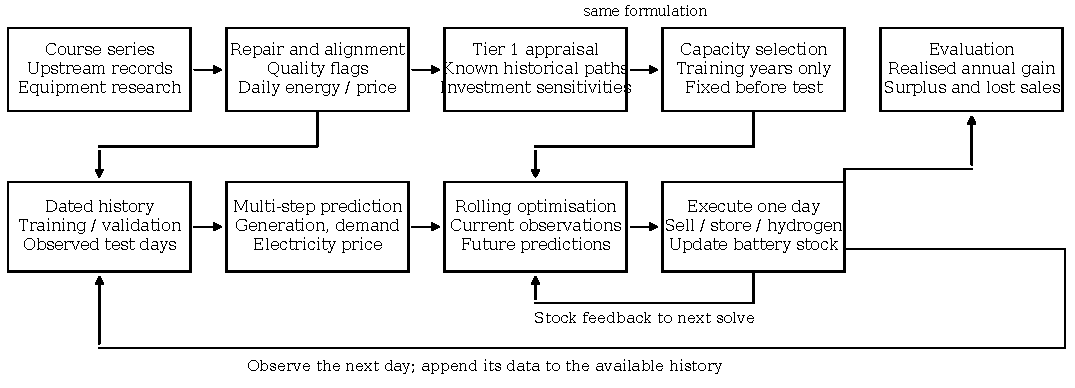
\includegraphics[width=\linewidth]{figures/model_architecture.pdf}
\caption{Study architecture. Tier 1 uses known historical paths. Tier 2B uses
past observations for forecasting and carries physical storage state forward;
its investment decision precedes the test period.}
\label{fig:architecture}
\end{figure}

\section{Data audit and reconstruction}\label{sec:data}
The five supplied files contain fuel-level generation, its total, simulated
wind-farm generation, demand and market index prices. The fuel total is
checked against its components; it is not added to them again. The separate
simulated farm is added to that total as the declared asset boundary.
Generation and demand are daily mean powers in MW, converted to MWh by
multiplying by 24. We retain 1 January 2020--17 September 2026: 2,452 days
in Coordinated Universal Time (UTC). Source checks use Elexon records and
National Energy System Operator (NESO) series.

\begin{table}[H]
\centering\small
\caption{Detected problems, evidence and repair. Date counts can overlap.}
\begin{tabularx}{\linewidth}{@{}P{.27\linewidth}Y@{}}
\toprule
Problem and extent & Identification and reconstruction \\
\midrule
Eight non-wind/solar fuels zero on 107 days; solar zero on 42 days &
Synchronous zeros conflict with archived records. Reaggregate Elexon actual
generation by production type; use calibrated fuel half-hour or NESO solar
series when that source is incomplete. Interpolate short gaps. \\
Midnight query endpoints: 7 generation, 350 demand, 346 price dates &
Original values reproduce the first timestamp rather than the full day.
Retrieve the complete UTC day and recalculate its mean. \\
Missing dates: 30 generation, 1 demand, 30 price &
Calendar gaps are verified against the dated upstream series. Restore those
records where available; otherwise use flagged whole-day estimates. \\
Invalid demand slots &
Some five-minute records are below 10,000 MW, including 636 MW on 2 August
2022. Retain valid slots and reconstruct others
from calibrated NESO demand; flag whole-day estimates. \\
Zero-volume price placeholders &
115,571 provider records have no traded volume. Exclude those placeholders,
volume-weight active providers within each half-hour, then average the day.
Retain genuine zero and negative prices. \\
\bottomrule
\end{tabularx}
\label{tab:repair}
\end{table}

The repaired files share a complete calendar; fuel components sum to total
generation, and the two price-unit columns retain their factor of 24.
The 2 August demand mean is reconstructed as 28,744 MW. The audit identifies
436 dates with interpolation or estimation, 323 with cross-source
reconstruction and 1,929 satisfying the strict quality flag; categories
overlap \cite{repair}. The full set supports the primary analysis; the strict
subset is a sensitivity check. All original values, replacements, source
records and quality flags are retained. Historical prices are converted
to 2020 pounds using monthly consumer price indices \cite{cpi}.

\section{Common notation and assumptions}\label{sec:global}
Only quantities shared by both tiers are defined here. Equipment decisions,
dispatch policies, forecast information and technical parameters are
introduced in their respective chapters.
\begin{table}[H]
\centering\small
\caption{Notation shared across the study.}
\begin{tabularx}{\linewidth}{@{}lY r@{}}
\toprule
Symbol & Meaning & Unit \\
\midrule
\(t\in\mathcal T\) & UTC day in the selected study period & day \\
\(G_t,D_t\) & Available generation and market demand (sales ceiling) & MWh \\
\(p_t\) & Market electricity price, in constant 2020 pounds & \gbp/MWh \\
\(S_t\) & Physical surplus, \(\max(G_t-D_t,0)\) & MWh \\
\(Y\) & Represented years: sum of each sampled day's calendar-year fraction & year \\
\bottomrule
\end{tabularx}
\end{table}
The supplied series describe a constructed system rather than observed
network congestion \cite{brief,teacher}. Existing generation is fixed;
its unchanged costs cancel in investment comparisons. Demand limits sales
and is not an additional unpaid internal load. We assume no electricity
imports, no additional export outlet and no payment for unused generation.
Spatial transfer limits are omitted. All monetary comparisons use constant
2020 pounds. These conventions are common to both tiers.

\chapter{Tier 1: deterministic investment appraisal}\label{chap:tier1}
\section{Problem analysis}\label{sec:problem1}
We select battery and electrolyser capacities and their daily use over
2020--25 (2,192 consecutive days). The investment is made once and applies
to all six years. Direct electricity sales provide the no-investment
benchmark. The investment case depends on three questions: whether
electrolysis can use electricity that could otherwise be sold, how much
hydrogen a buyer can take, and whether storage can shift enough electricity
to recover its costs.

\section{Assumptions and research}\label{sec:research1}
\subsection{Tier-specific assumptions}
\emph{Policy A} allocates electricity by economic value.
\emph{Policy B} serves current electricity demand first with generation
and then with stored electricity. B honours this priority even at negative
prices. Hydrogen is sold as produced subject to a common daily offtake limit.
Battery electricity can feed electrolysis after any applicable sales
priority. The daily model carries battery inventory forward, with at most
one net charge or discharge per model per day and zero opening and closing usable
inventory over the study period. Daily operation uses the historical paths.

We distinguish a broad market case and two smaller buyer cases.
The broad cap of 1,559 t/day is the highest UK annual hydrogen consumption
estimate in the 2022--24 source divided by the number of days in that year.
The 1.56 and 10 t/day cases illustrate smaller outlets.
Netback is the revenue per kg after non-electricity variable costs.
We take \gbp 7.80/kg as a scenario, rebasing the UK policy benchmark of
\gbp 175/MWh in 2012 pounds using 39.4 kWh/kg and the consumer price index.
The national total includes existing uses and provides a scale comparison
for the constructed system \cite{har,eho,cpi,basis}.

\subsection{Research objectives and parameter selection}
\begin{table}[H]
\centering\small
\caption{Physical and financial inputs. Monetary values are in 2020 pounds.}
\label{tab:research}
\begin{tabularx}{\linewidth}{@{}P{.19\linewidth}YY@{}}
\toprule
Input & Model specification & Basis and use \\
\midrule
Battery options &
Four Sungrow, Huawei and Tesla models, 0.215--3.854 MWh and
0.108--1.927 MW per unit. Round-trip efficiency is 90--92\%,
state of charge is limited to 20--80\%, and life is 15 years. &
Supplier data for performance. Course and Danish Energy Agency costs for
the smaller units and a public Tesla installed quote for the large unit.
Capital is \gbp 55,129--1,239,440 per unit and annual fixed operation is
\gbp 1,599--30,986 \cite{brief,dea,v6}. \\
Electrolyser options &
Eight ITM and Nel models, 1.31--50.31 MW. Specific consumption is
55.9--59.0 kWh/kg and the minimum online load is 10--25\%, by model. &
Manufacturer operating data. Common installed cost of \gbp 1.46m/MW
lets us compare size and efficiency on the same financial basis \cite{iea,v6}. \\
Electrolyser upkeep &
\gbp 25,862/MW-year fixed operation, \gbp 489,609/MW per stack renewal in
years 11 and 22, 30-year life. &
UK cost study. A second case uses its complete cost basis with a reserve
per kg of output in place of scheduled stack renewal \cite{beis,v6}. \\
Financial treatment &
5\% real discount rate, zero residual value and battery commissioning charge. &
Costs enter as annual equivalents. The 20\% starting state of charge is
accounted for through commissioning \cite{basis,v6}. \\
\bottomrule
\end{tabularx}
\end{table}

\newpage
\section{Mathematical model}\label{sec:model1}
Indices \(i\) and \(j\) denote battery and electrolyser models.
All daily energy flows and inventories are in MWh. Installed counts
\(b_i,n_j\) and online electrolyser counts \(z_{jt}\) are nonnegative
integers. The daily variables are direct sales \(q_t\), generation sent
directly to electrolysis \(g_t^H\), battery charge \(c_{it}\),
discharge for sales \(r_{it}\) and for electrolysis \(u_{it}\), usable stock
\(s_{it}\), and electrolyser input \(h_{jt}\). The conversion factor
\(\kappa_j\) is MWh/kg and \(L\) is the daily offtake limit in kg.
With netback \(v\) in \gbp/kg and annual equipment costs \(a_i^B,a_j^H\),
we maximise annual equivalent profit
\begin{equation}
\max\quad \Pi =
\frac{1}{Y}\sum_{t\in\mathcal T}
\left[p_t\left(q_t+\sum_i r_{it}\right)+
\sum_j (v-w_j)\frac{h_{jt}}{\kappa_j}\right]
-\sum_i a_i^B b_i-\sum_j a_j^H n_j .
\label{eq:profit}
\end{equation}
Here \(w_j\) is the variable stack reserve in \gbp/kg, zero when
stack renewal is charged through the annual equipment cost.

The daily flow equations allocate generation, cap total sales at market
demand and balance both sources of electricity into electrolysis:
\begin{align}
 q_t+g_t^H+\sum_i c_{it}&\le G_t, &
 q_t+\sum_i r_{it}&\le D_t, &
 \sum_j h_{jt}&=g_t^H+\sum_i u_{it}. \label{eq:flow}
\end{align}
The unallocated part of generation is unused. For battery \(i\), \(W_i\)
is the usable energy per unit, \(P_i\) the power in MW, and \(\eta_i\)
the square root of round-trip efficiency. The inventory and daily throughput
constraints are
\begin{align}
s_{it}&=(1-\delta_i)s_{i,t-1}+\eta_i c_{it}-(r_{it}+u_{it})/\eta_i,
 & 0\le s_{it}&\le W_i b_i, \label{eq:stock}\\
c_{it}&\le b_i\min(24P_i,W_i/\eta_i),
 & r_{it}+u_{it}&\le b_i\min(24P_i,\eta_i W_i). \label{eq:window}
\end{align}
Daily self-discharge \(\delta_i\) is zero in the main case. We set
\(s_{i0}=s_{iT}=0\) for \(T=|\mathcal T|\), and at least one of \(c_{it}\)
and \(r_{it}+u_{it}\) is zero. A binary charge-mode indicator enforces
this choice when needed. For electrolysis, \(H_j\) is the full-load daily
input per unit and \(\alpha_j\) its minimum operating fraction:
\begin{align}
\alpha_j H_j z_{jt}\le h_{jt}&\le H_j z_{jt}, &
z_{jt}&\le n_j, &
\sum_j h_{jt}/\kappa_j&\le L. \label{eq:hydrogen}
\end{align}
All flows are nonnegative. With \((x)_+=\max(0,x)\), B also imposes
\begin{equation}
q_t=\min(G_t,D_t), \qquad
\sum_i r_{it}=\min\!\left\{(D_t-G_t)_+,\,
            \sum_i\eta_i(1-\delta_i)s_{i,t-1}\right\}.
\label{eq:priority}
\end{equation}
The short-duration battery models can discharge all usable stock within
a day. A binary indicator selects the binding branch of the minimum.

For a unit with capital \(K\), fixed annual operating cost \(F\), lifetime
\(N\), real discount rate \(d\) and renewals \(C_k\) in years \(k\),
annual cost is
\begin{equation}
a=F+\frac{d}{1-(1+d)^{-N}}
\left(K+\sum_k\frac{C_k}{(1+d)^k}\right).
\label{eq:annualcost}
\end{equation}
Reported gain subtracts each policy's own optimum with all \(b_i,n_j=0\).

\textbf{Numerical checks.}
HiGHS certified the 14 portfolio cases with a maximum reported relative
gap below \(10^{-9}\). Independent checks reproduced balances, cash
flows and zero-battery dispatch. Six forced-storage cases tested stock
carry-over, discharge to electrolysis and B's priority rule \cite{v6}.

\newpage
\section{Results and analysis}\label{sec:results1}
\subsection{Capacity and historical performance}
In the broad market case, electrolysis-only and joint investment return
the same portfolios. A selects 3,631 MW (721 Neptune V and two Neptune II
units) and B selects 740 MW (147 Neptune V units). At 10 t/day, both choose
23.4 MW across six smaller modules. Initial capital in the broad case is
\gbp 5.30bn (A) and \gbp 1.08bn (B), producing about 488,000 and
19,100 t/year of hydrogen respectively.
\begin{table}[H]
\centering\small
\caption{Six-year portfolio choices and annual profit gains by policy.
A dash marks an excluded investment. Gains are in \gbp m/year.}
\label{tab:annual}
\textit{(a) Allowed assets at the broad market cap}\par\vspace{2pt}
\begin{tabular}{@{}l r r r r r r@{}}
\toprule
 & \multicolumn{3}{c}{Policy A} & \multicolumn{3}{c}{Policy B} \\
\cmidrule(lr){2-4}\cmidrule(l){5-7}
Allowed investment & Battery & Electrolysis & Gain & Battery & Electrolysis & Gain \\
 & (MWh) & (MW) & & (MWh) & (MW) & \\
\midrule
Battery only & 0 & -- & 0 & 0 & -- & 0 \\
Electrolysis only & -- & 3,631 & 1,639 & -- & 740 & 37.71 \\
Joint choice & 0 & 3,631 & 1,639 & 0 & 740 & 37.71 \\
\bottomrule
\end{tabular}
\par\vspace{5pt}
\textit{(b) Smaller outlets with both assets allowed}\par\vspace{2pt}
\begin{tabular}{@{}l r r r r r@{}}
\toprule
Daily offtake & Battery & \multicolumn{2}{c}{Electrolysis (MW)} &
 \multicolumn{2}{c}{Gain} \\
\cmidrule(lr){3-4}\cmidrule(l){5-6}
(t/day) & (MWh), A/B & A & B & A & B \\
\midrule
1.56 & 0 & 3.84 & 3.84 & 1.91 & 0.35 \\
10 & 0 & 23.42 & 23.42 & 12.68 & 2.44 \\
\bottomrule
\end{tabular}
\end{table}

At 10 t/day, B loses money in 2021, 2023 and 2024, with a worst
year of \gbp 1.26m below no investment. These years have 43, 29 and
30 surplus days, respectively, against 154 in 2022. A can produce on
additional days when the hydrogen value exceeds
the price of forgone electricity sales. At the broad cap, A meets 82.2\%
of electricity demand and B meets 92.2\%. Using the alternative UK cost
basis at that cap leaves A's capacity unchanged and raises B's from
740 to 1,465 MW, with zero batteries in both cases \cite{beis,v6}.

\subsection{Energy attribution and contract sensitivity}\label{sec:contract1}
The historical mean physical surplus is 2,276 GWh/year.
For the zero-battery solutions we attribute \(\min(g_t^H,S_t)\) to physical
surplus first. The remaining electrolysis input uses energy within current
electricity demand. We calculate the monetary loss separately against
same-policy electricity sales without investment, accounting for negative
prices under A. The aggregate records identify the available fuels by day
and cannot trace the generating unit that supplied electrolysis.
\begin{table}[H]
\centering\small
\caption{Electrolysis sourcing and forgone electricity receipts.
Energy is in GWh/year. The revenue reduction is in \gbp m/year.}
\label{tab:attribution}
\begin{tabular}{@{}l c r r r r@{}}
\toprule
Offtake & Policy & \shortstack{Total input} & \shortstack{Physical\\surplus} &
\shortstack{Within current\\demand} & \shortstack{Electricity\\revenue reduction} \\
\midrule
Broad & A & 27,255 & 2,184 & 25,070 & 1,618 \\
Broad & B & 1,067 & 1,067 & 0 & 0 \\
10 t/day & A & 183 & 43 & 140 & 9.18 \\
10 t/day & B & 43 & 43 & 0 & 0 \\
\bottomrule
\end{tabular}
\end{table}

In the broad market case, A uses about 2,184 GWh/year of physical surplus,
only 8\% of its total electrolysis input. Its electricity receipts fall by
\gbp 1,618m/year. B uses 1,067 GWh/year of surplus and preserves direct
sales, limiting its hydrogen throughput. At 10 t/day, each captures
about 43 GWh/year, just under 2\% of the physical surplus.

\newpage
\noindent
After reoptimising electrolysis and dispatch, the lowest netbacks that
support any investment are about \gbp 3.32/kg in A and \gbp 4.57/kg in B
at 10 t/day. At 1.56 t/day they rise to \gbp 3.38/kg and \gbp 4.66/kg.
The 23.4 MW portfolio in Table~\ref{tab:annual} is sized at \gbp 7.80/kg.
Holding its operation fixed, it breaks even at \gbp 3.90/kg in A or
\gbp 4.61/kg in B. At other prices, reoptimise operation and capacity.

\subsection{Storage and investment sensitivity}\label{sec:storage1}
\begin{table}[H]
\centering\small
\caption{Storage entry under historical and stressed conditions.
Price multipliers scale the standard deviation of daily prices.}
\label{tab:storage}
\begin{tabularx}{\linewidth}{@{}P{.35\linewidth}Y@{}}
\toprule
Test & Implication for storage investment \\
\midrule
Historical high-volatility windows &
All four battery options remain unselected in the highest-variance
60-, 90-, 180- and 365-day windows under both policies. The 90-day price
standard deviation is \gbp 114/MWh against \gbp 65/MWh over six years. \\
Battery cost and price stress &
Halving purchase and maintenance costs still gives zero batteries.
With historical supply and demand, batteries first enter at about
\(40\times\) (A) and \(127\times\) (B) the historical price standard
deviation at the modelled costs. \\
Joint supply and price stress &
The joint grid selects zero batteries at the historical price dispersion
across nine supply--demand gap dispersions. At \(120\times\) price
dispersion in B, raising gap dispersion from \(1\times\) to \(1.1\times\)
changes the optimum from zero to 2.60 GWh. \\
Cavern compressed air &
A separate 50 MW / 1.5 GWh test, at one-third of the reference battery
installation cost per MWh and 62\% round-trip efficiency, needs
\(5.38\)--\(5.50\times\) (A) or \(15.00\)--\(15.13\times\) (B) price
dispersion at the original supply--demand gap. \\
\bottomrule
\end{tabularx}
\end{table}
The volatility tests centre each series before scaling, preserving
means and date order. The battery and cavern tests allow the electrolyser
choice to adjust. For battery-only investment, even free charging and
the full usable discharge on every positive-price day yield at most
57\% of annual ownership cost across the four models. At historical
prices the cavern's annual operating
gain is \gbp 1.38m in A and \gbp 2.35m in B, against an annual cost of
\gbp 8.52m \cite{stress}.

\subsection{Investment recommendations}\label{sec:recommendations1}
\textbf{Size electrolysis to secured demand.}
For 10 t/day, appraise the 23.4 MW portfolio against the \gbp 34.2m
initial cost. A and B yield \gbp 12.68m and \gbp 2.44m/year respectively
(Table~\ref{tab:annual}). Confirm the ability to displace electricity
sales before relying on A. Under B, use the observed loss years to test
cash reserves and the case for staged procurement. Reduce the appraisal to roughly
3.84 MW if the outlet is near 1.56 t/day. At a netback below the
market entry levels above, defer electrolysis at the tested costs.
The broad cap describes market scale. Capacity at that scale warrants
appraisal only with much larger contracted offtake.

\textbf{Defer daily storage.}
Both cost and historical stress tests support zero batteries
(Table~\ref{tab:storage}). Reopen procurement if a lower installed cost
or additional revenue brings the expected operating gain above annual
ownership costs. For the cavern, the historical gain implies an annual
cost ceiling of \gbp 1.38m under A or \gbp 2.35m under B on these inputs.

\chapter{Tier 2B: forecasting and chronological operation}\label{chap:tier2}
\section{Information and experimental design}\label{sec:design2}
The operating decision is made once per day. Following the classroom
simplification, current-day generation, demand and price are known at that
decision, while future days are unknown \cite{teacher}. Let
\(y_t=(G_t,D_t,p_t)\) and let \(\mathcal I_t\) contain observations through
day \(t\), the installed equipment and the previous day's usable stock.
Only information in \(\mathcal I_t\) can determine the implemented action.
Current-day aggregates are treated as observed at this daily planning decision.

We reserve 2020--22 for training and capacity selection, 2023 for model and
horizon selection, and 2024--25 for the final test. A forecasting training
target must lie before its corresponding cutoff. Repair calibration, scaling and hyperparameter
selection use training/validation data only. The six-year Tier 1 capacity
comparison remains a hindsight benchmark; test observations must not
choose the capacity used in the predictive experiment.

\section{Multi-step forecasting model}\label{sec:forecast2}
The proposed first predictive model is regularised linear autoregression,
compared against a seven-day seasonal-naive predictor. At each forecast
origin \(t\), the feature vector \(f_t\) contains observed generation,
demand and price lags, day-of-week indicators and annual sine/cosine terms.
For variable \(j\in\{G,D,p\}\) and horizon \(k=1,\ldots,H\), fit
\begin{equation}
\widehat\beta_{jk}=\arg\min_{\beta}
\sum_{\tau\in\mathcal A_k}(y_{\tau+k,j}-f_\tau^{\top}\beta)^2
+\lambda\lVert\beta\rVert_2^2,
\qquad
\widehat y_{t+k,j}=f_t^{\top}\widehat\beta_{jk},
\end{equation}
where \(\mathcal A_k\) contains eligible training origins whose targets
are already observed, \(\lambda\ge0\) is the validation-selected penalty
and \(H\) is the planning horizon. Forecast generation and demand are
projected onto nonnegative values; negative price forecasts remain allowed.
The seasonal-naive forecast uses the most recent observation with the same
weekday, recursively if needed.

\section{Rolling optimisation and storage feedback}\label{sec:rolling2}
At day \(t\), installed battery and electrolyser counts are fixed. A
planning problem uses observed values for the current day and predictions
for \(t+1,\ldots,t+H\). It retains the Tier 1 flow, demand, throughput and electrolysis
constraints, but replaces the pooled energy balance with chronological stock:
\begin{equation}
s_\tau=s_{\tau-1}+\eta c_\tau-r_\tau/\eta,
\qquad 0\le s_\tau\le E_Bb,
\qquad \tau=t,\ldots,t+H.
\end{equation}
Here \(s_{t-1}\) is the measured initial stock for that solve. The optimiser
maximises forecast operating receipts plus a terminal-stock value; the latter
is selected on validation data to avoid repeatedly liquidating storage at an
artificial short horizon. Only \((q_t,c_t,r_t,h_t)\) is implemented. Its
realised stock becomes the next solve's initial condition. The test's initial
and final stock treatment is held equal across all compared policies.

\section{Evaluation and results to be completed}\label{sec:evaluation2}
Forecast error is reported by series and horizon using mean absolute error
and root mean square error, with price errors in \gbp/MWh and physical
errors in MWh. Operating evaluation compares the predictive controller,
the same controller with seasonal-naive forecasts, a current-day rule and
a full-path perfect-information optimiser, all at identical installed
capacities and with identical data, costs and terminal stock. The gap to
perfect information measures the realised loss from restricted information,
rather than a change in investment scale.

Since zero batteries remove cross-day storage, fixed nonzero battery cases
will diagnose prediction and feedback value alongside the training-selected
investment. Results will include forecast errors, realised annual value,
surplus capture, lost sales, stock feasibility and seasonal/adverse-period
comparisons. These forecast and control experiments are pending.

\label{body-last}
\clearpage
\setcounter{page}{1}
\renewcommand{\thepage}{R\arabic{page}}
\begin{thebibliography}{10}
\addcontentsline{toc}{chapter}{References}
\small\setlength{\itemsep}{3pt}\setlength{\parskip}{0pt}
\bibitem{brief} MMCS (2026). \emph{2026/27 Project Brief}, pp. 1--6.
\bibitem{teacher} MMCS (2026). \emph{Project launch lecture}, timestamped
transcript, 26 October, 01:09--01:24; and documented discussion clarifications.
\bibitem{repair} Group 15 (2026). \emph{Full data repair, 20261104-v2}.
Source evidence, cell audit and validation archive. Repository commit
\texttt{53e3b50}; included in the accompanying package.
\bibitem{cpi} Office for National Statistics.
\href{https://www.ons.gov.uk/economy/inflationandpriceindices/timeseries/d7bt/mm23}
{\emph{Consumer Prices Index, series D7BT}}.
\bibitem{dea} Danish Energy Agency.
\href{https://ens.dk/media/6589/download}{\emph{Technology data for energy storage}},
sheet 180.
\bibitem{iea} International Energy Agency (2025).
\href{https://www.iea.org/reports/global-hydrogen-review-2025/executive-summary}
{\emph{Global Hydrogen Review 2025}}, installed electrolyser costs.
\bibitem{beis} Department for Business, Energy and Industrial Strategy (2021).
\href{https://assets.publishing.service.gov.uk/media/611b710e8fa8f53dc994e59d/Hydrogen_Production_Costs_2021.pdf}
{\emph{Hydrogen Production Costs 2021}} and assumptions annex.
\bibitem{har} Department for Energy Security and Net Zero (2023).
\href{https://www.gov.uk/government/publications/hydrogen-production-business-model-net-zero-hydrogen-fund-shortlisted-projects/hydrogen-production-business-model-net-zero-hydrogen-fund-har1-successful-projects}
{\emph{Hydrogen Allocation Round 1 successful projects}}.
\bibitem{basis} Group 15 (2026). \emph{Financial conversions and parameter basis}.
ECB exchange-rate and ONS inflation conversions; R1--R4 research and
\texttt{research/PARAMETER\_BASIS.md} in the accompanying package.
\bibitem{peer} Group 15 (2026). \emph{Independent implementation B: annual
replay results}. Repository commit \texttt{53e3b50};
\texttt{references/independent-b-cases.csv} in the accompanying package.
\bibitem{eho} European Hydrogen Observatory (2025).
\href{https://observatory.clean-hydrogen.europa.eu/hydrogen-landscape/end-use/hydrogen-demand}
{\emph{Hydrogen Demand}}, 2025 update, 2022--24 UK end-use totals.
\bibitem{v6} Group 15 (2026). \emph{Tier 1 v6 equipment and investment study}.
10 November working archive. Product inputs and their sources, audited
daily schedules and investment comparisons.
\bibitem{stress} Group 15 (2026). \emph{Tier 1 storage sensitivity}.
11--12 November working archive. Equipment-cost, joint-volatility,
historical-window and cavern-storage tests.
\end{thebibliography}

\end{document}
